\documentclass[english]{beamer}\usepackage[]{graphicx}\usepackage[]{xcolor}
% maxwidth is the original width if it is less than linewidth
% otherwise use linewidth (to make sure the graphics do not exceed the margin)
\makeatletter
\def\maxwidth{ %
  \ifdim\Gin@nat@width>\linewidth
    \linewidth
  \else
    \Gin@nat@width
  \fi
}
\makeatother

\definecolor{fgcolor}{rgb}{0.345, 0.345, 0.345}
\newcommand{\hlnum}[1]{\textcolor[rgb]{0.686,0.059,0.569}{#1}}%
\newcommand{\hlsng}[1]{\textcolor[rgb]{0.192,0.494,0.8}{#1}}%
\newcommand{\hlcom}[1]{\textcolor[rgb]{0.678,0.584,0.686}{\textit{#1}}}%
\newcommand{\hlopt}[1]{\textcolor[rgb]{0,0,0}{#1}}%
\newcommand{\hldef}[1]{\textcolor[rgb]{0.345,0.345,0.345}{#1}}%
\newcommand{\hlkwa}[1]{\textcolor[rgb]{0.161,0.373,0.58}{\textbf{#1}}}%
\newcommand{\hlkwb}[1]{\textcolor[rgb]{0.69,0.353,0.396}{#1}}%
\newcommand{\hlkwc}[1]{\textcolor[rgb]{0.333,0.667,0.333}{#1}}%
\newcommand{\hlkwd}[1]{\textcolor[rgb]{0.737,0.353,0.396}{\textbf{#1}}}%
\let\hlipl\hlkwb

\usepackage{framed}
\makeatletter
\newenvironment{kframe}{%
 \def\at@end@of@kframe{}%
 \ifinner\ifhmode%
  \def\at@end@of@kframe{\end{minipage}}%
  \begin{minipage}{\columnwidth}%
 \fi\fi%
 \def\FrameCommand##1{\hskip\@totalleftmargin \hskip-\fboxsep
 \colorbox{shadecolor}{##1}\hskip-\fboxsep
     % There is no \\@totalrightmargin, so:
     \hskip-\linewidth \hskip-\@totalleftmargin \hskip\columnwidth}%
 \MakeFramed {\advance\hsize-\width
   \@totalleftmargin\z@ \linewidth\hsize
   \@setminipage}}%
 {\par\unskip\endMakeFramed%
 \at@end@of@kframe}
\makeatother

\definecolor{shadecolor}{rgb}{.97, .97, .97}
\definecolor{messagecolor}{rgb}{0, 0, 0}
\definecolor{warningcolor}{rgb}{1, 0, 1}
\definecolor{errorcolor}{rgb}{1, 0, 0}
\newenvironment{knitrout}{}{} % an empty environment to be redefined in TeX

\usepackage{alltt}

%% The most common packages are already included in:
\usetheme{biostat}
%%%%%%%%%%%%%%%%%%%%%%%%%%%%%%%%%%%%%%%%%%%%%%%%%%%%%%%% 

%% Header data: (adjust to your needs:
\def\uzhunit{Master Thesis Biostatistics}             %% if (not) needed comment/uncomment
%\def\uzhunitext{STA480}
\title[Recruitment rate stochasticity
at the design stage of a clinical trial]{Frequentists and Bayesian methods to incorporate
recruitment rate stochasticity
at the design stage of a clinical trial}
%% Optional Argument in [Brackets]: Short Title for Footline

%% The following are all optional, simply comment them
\author{Supervision by Malgorzata Roos}
%\institute{Biostatistics Journal Club}  %% optional
\subtitle{Pilar Pastor}
%\date{\today}
%%%%%%%%%%%%%%%%%%%%%%%%%%%%%%%%%%%%%%%%%%%%%%%%%%%%%%%% 




%%%%%%%%%%%%%%%%%%%%%%%%%%%%%%%%%%%%%%%%%%%%%%%%%%%%%%%% 
\IfFileExists{upquote.sty}{\usepackage{upquote}}{}
\begin{document}
\maketitle
%%%%%%%%%%%%%%%%%%%%%%%%%%%%%%%%%%%%%%%%%%%%%%%%%%%%%%%% 
%% Start with slides here: put them between `\begin{frame}` and `\end{frame}`


\begin{frame}{Why recruitment rates?}

\begin{itemize}
\item Timely recruitment vital to the success of a clinical trial
\item Inadequate number of subjects $\rightarrow$ lack of power
\item Recruitment period too long $\rightarrow$ competing treatments
\item Recruitment of patients varies at each stage 
\item Accrual = Cumulative Recruitment
\item \cite{carter2004application}
\end{itemize}


\end{frame}


\begin{frame}{Target Population}

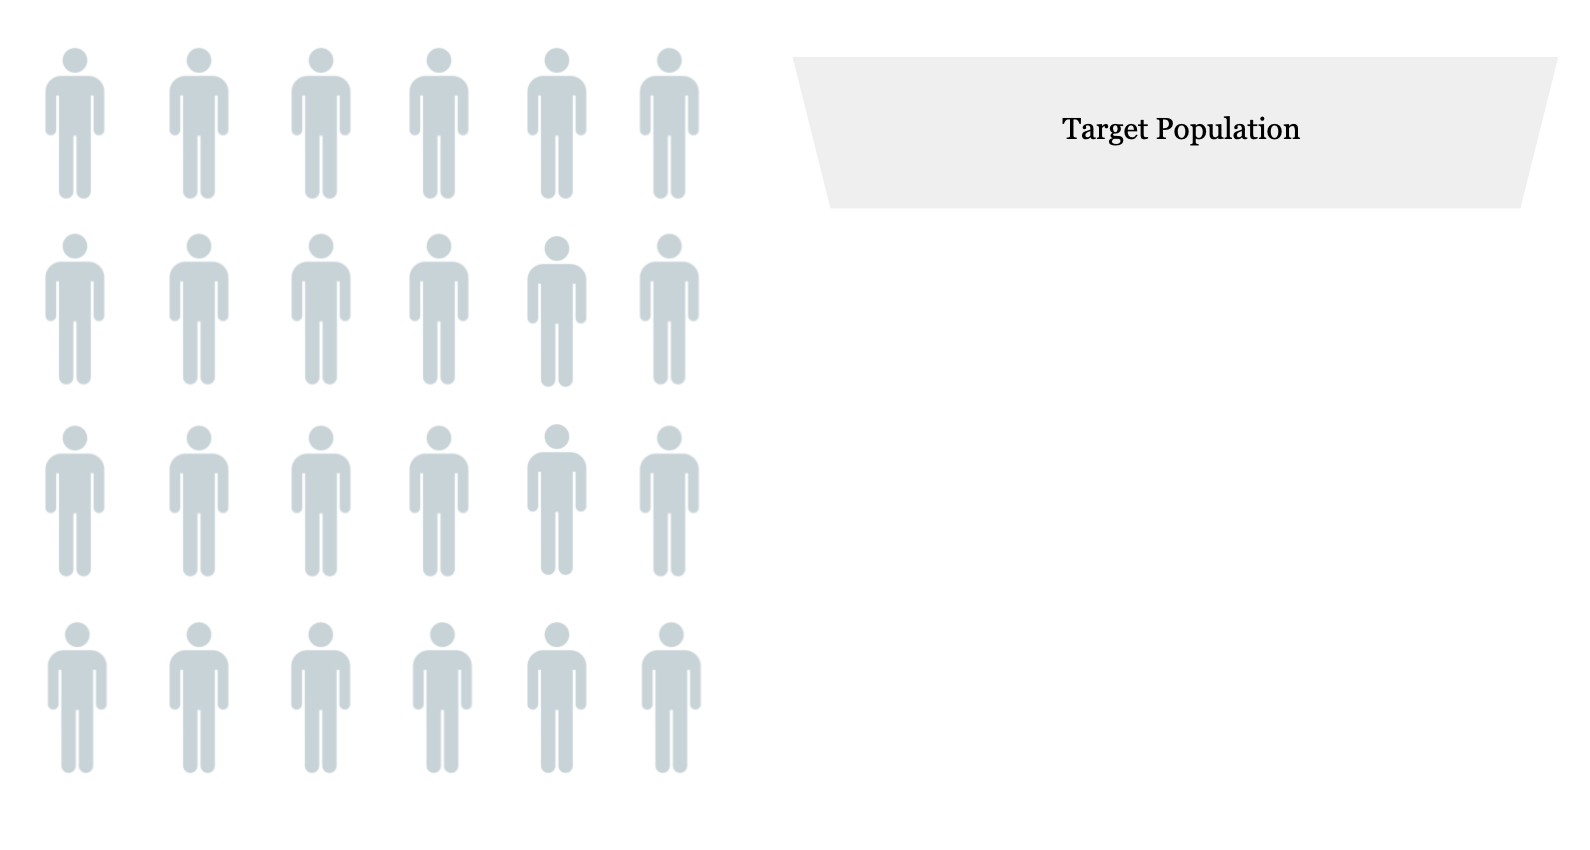
\includegraphics[width=100mm,scale=1]{targetpop.png}

\end{frame}

\begin{frame}{Eligibility}

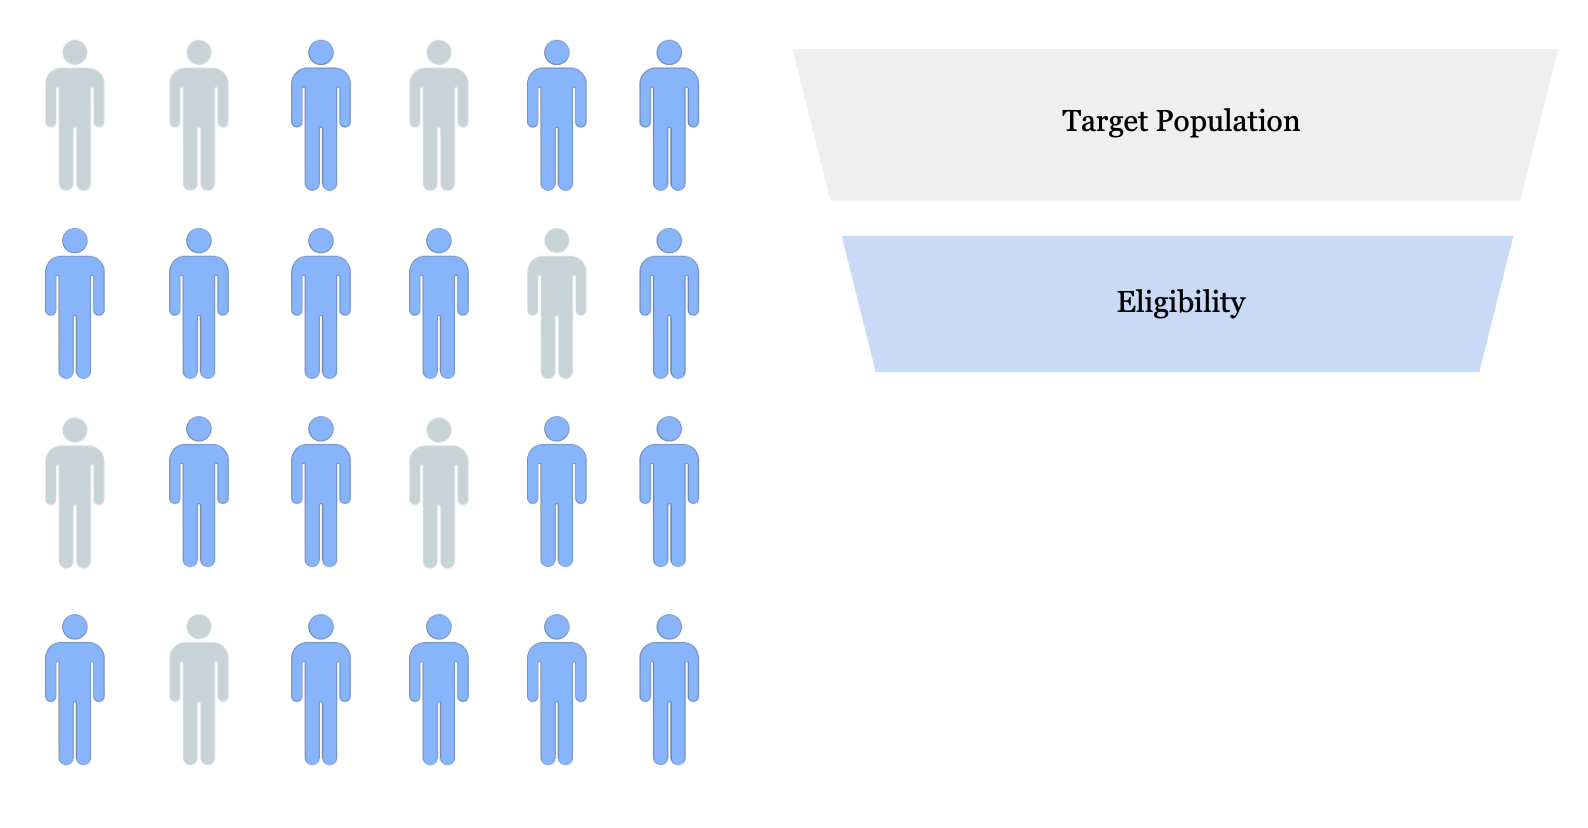
\includegraphics[width=100mm,scale=1]{eligibility.png}

\end{frame}

\begin{frame}{Enrollment}

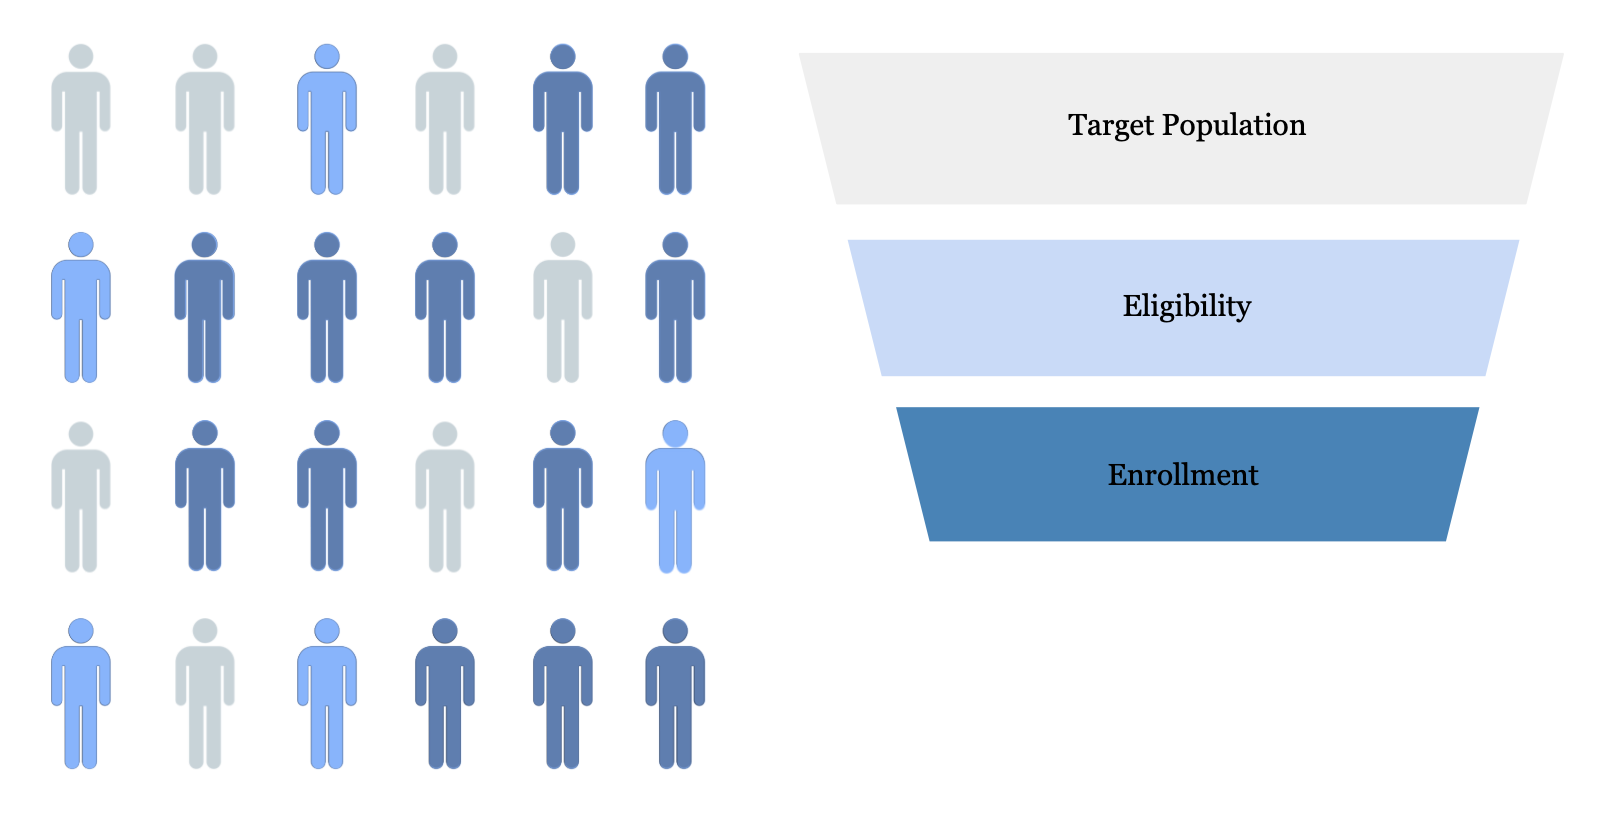
\includegraphics[width=100mm,scale=1]{enrollment.png}


\end{frame}

\begin{frame}{Randomization}

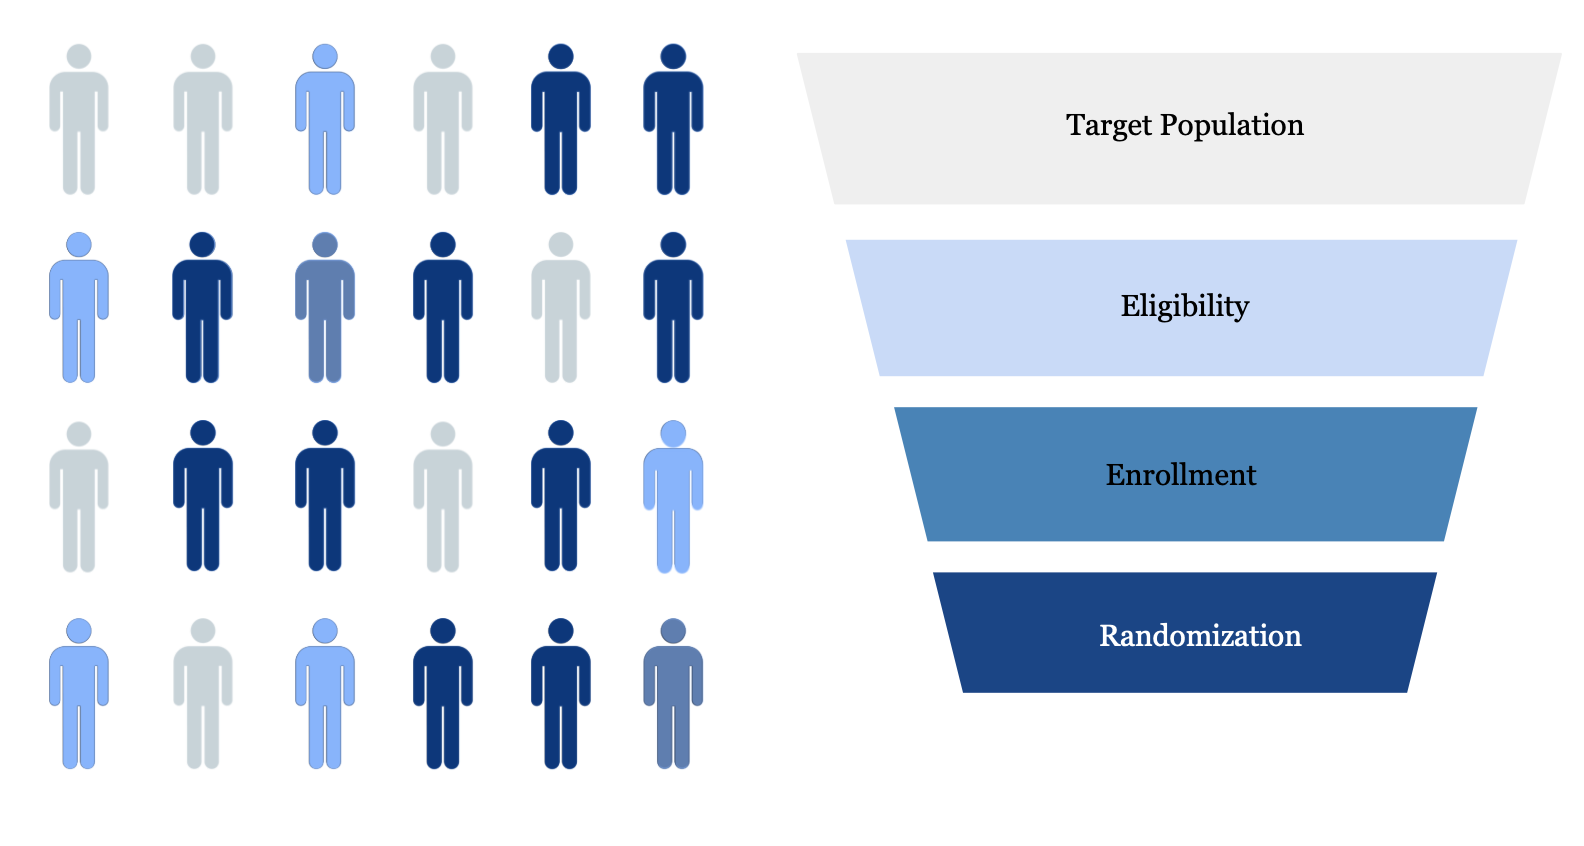
\includegraphics[width=100mm,scale=1]{randomization.png}

\end{frame}

\begin{frame}{Statistical Analysis}

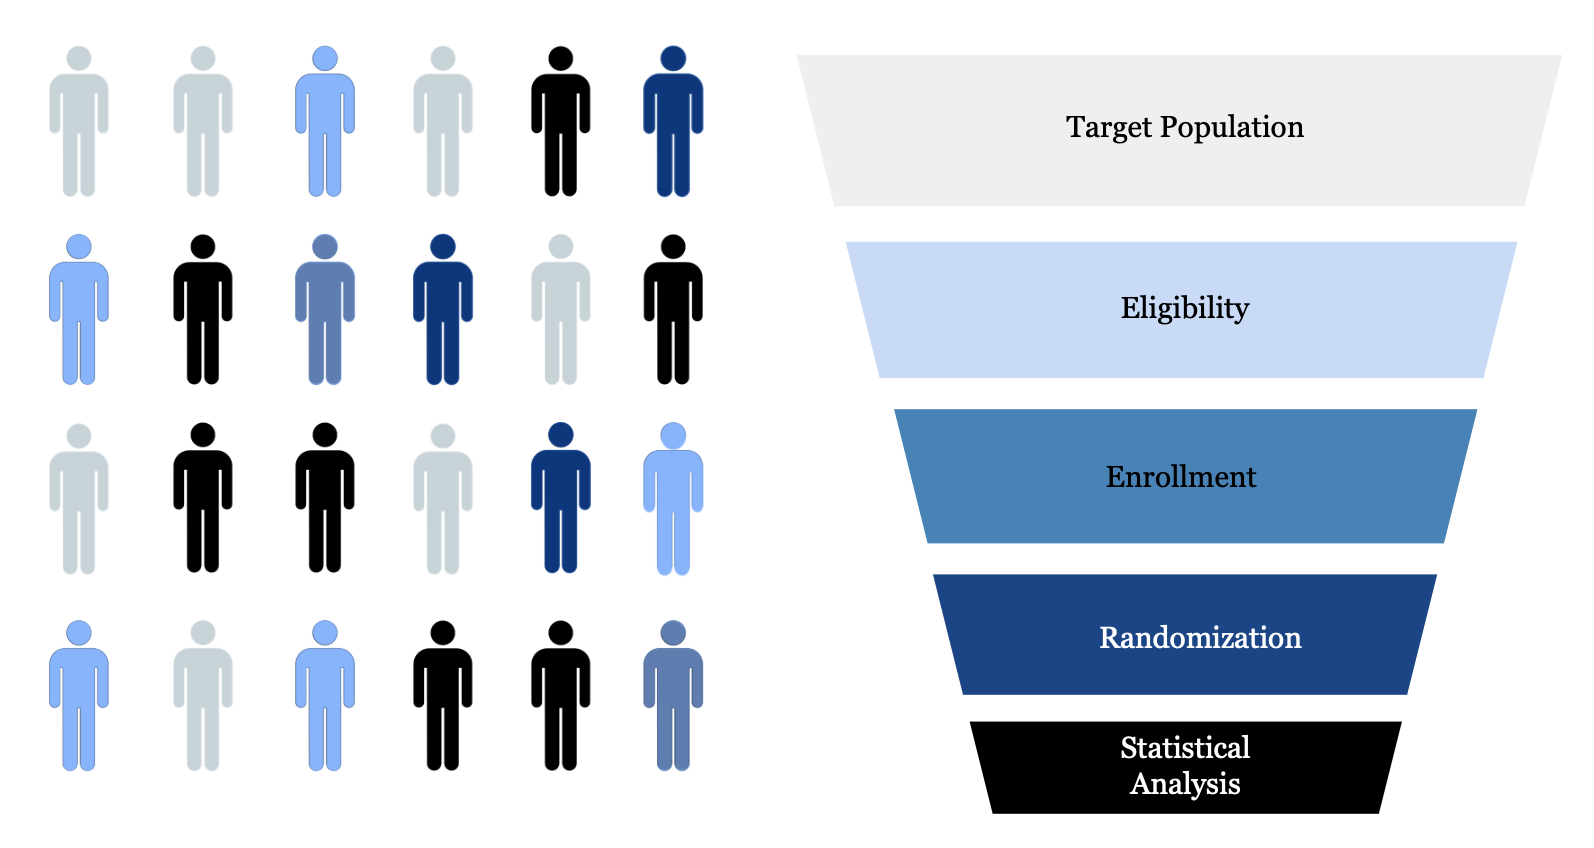
\includegraphics[width=100mm,scale=1]{statanal.png}

\end{frame}


\begin{frame}{Patient Leakage}

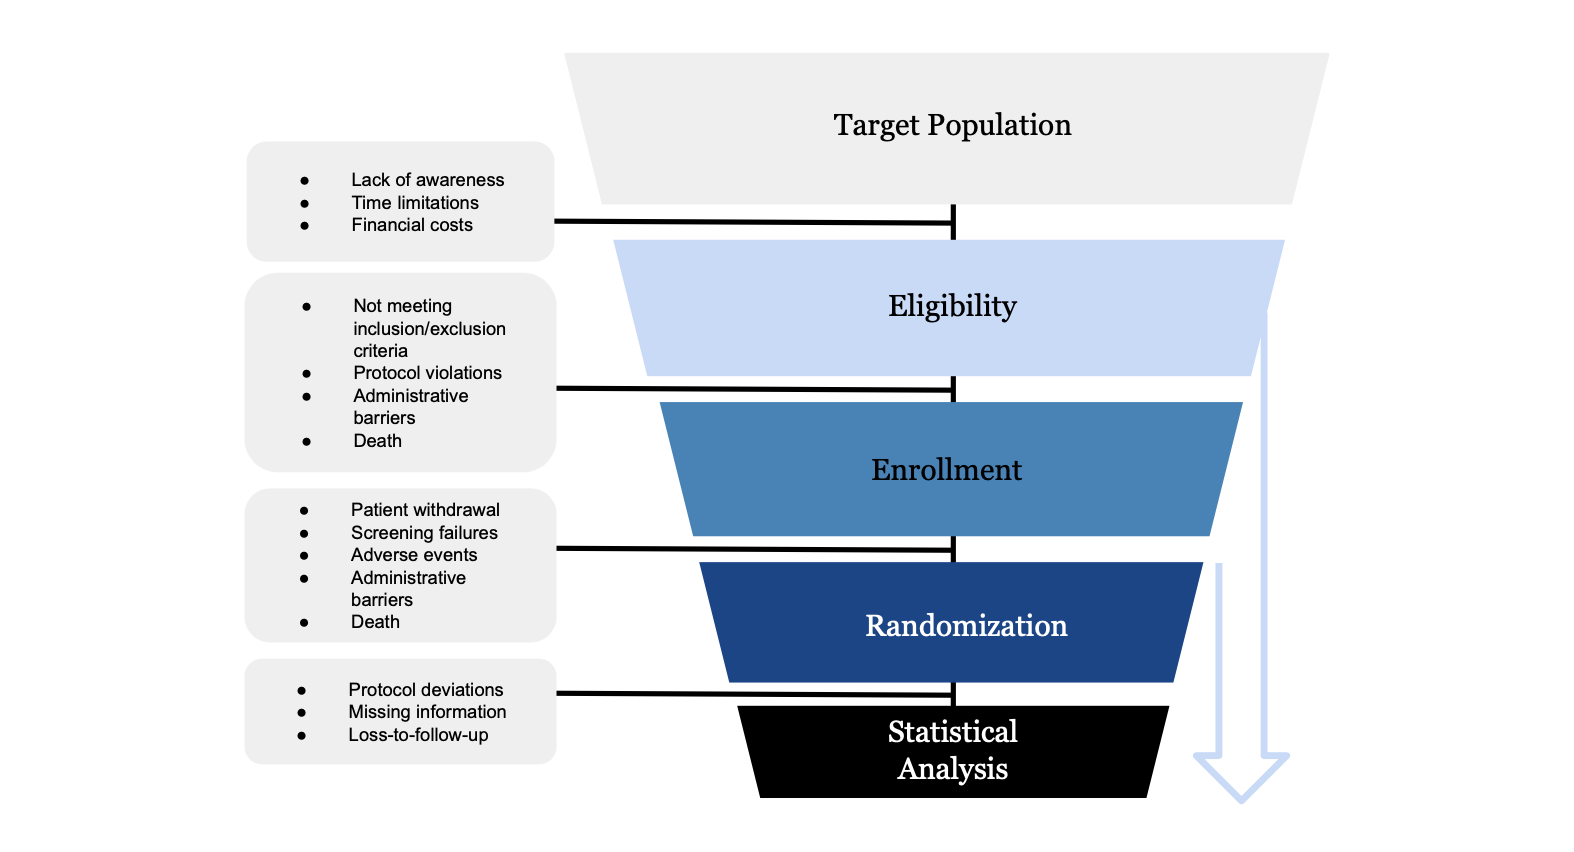
\includegraphics[width=100mm,scale=1]{attrition.png}

\end{frame}


\begin{frame}{Uncertainty}

\begin{itemize}
\item \textbf{Aleatory}: randomness inherent and unpredictable
\item \textbf{Epistemic}: arises from limited knowledge about parameters

\begin{figure}[h]
    \centering
    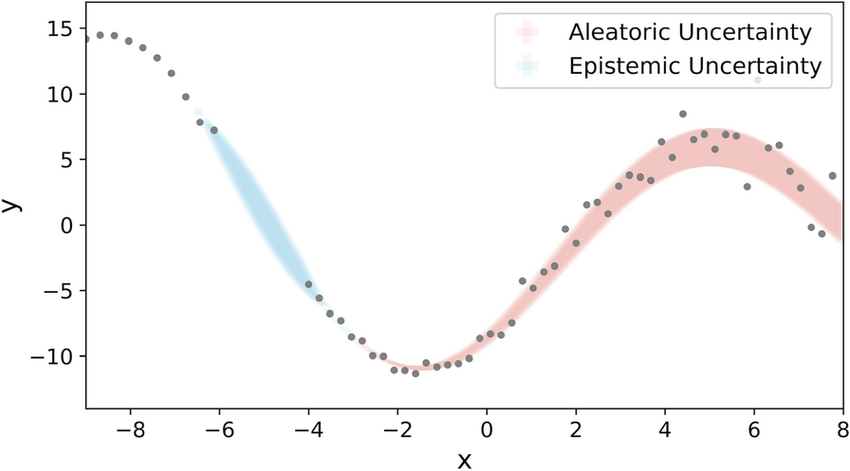
\includegraphics[width=60mm,scale=0.7]{illustration_uncertainty.png}
    \caption{Visualization of two types of uncertainty \citep{yang2023explainable}}
    \label{fig:uncertainty}
\end{figure}


\end{itemize}


\end{frame}

\begin{frame}{Models for Counts}

\begin{table}[h!]
\centering
\resizebox{\textwidth}{!}{
\begin{tabular}{cccccc}
 \textbf{Methods} & \textbf{Counts} & \textbf{Expectation} & \textbf{Variance} & \textbf{Aleatory} & \textbf{Epistemic} \\
\hline
\hline
Expectation & $C(t) = \lambda  t$ & $\lambda  t$ & 0 & No & No \\
Poisson & $C(t) \sim \textrm{Po} (\lambda  t)$ & $\lambda  t$ & $\lambda  t$ & Yes & No \\
Negative Binomial & $C(t) \sim \textrm{Po} (\Lambda  t)$; $\Lambda \sim \textrm{G}(\alpha,\beta)$ & $\frac{\alpha}{\beta}$ & $\frac{\alpha(\beta+1)}{\beta^2}$ & Yes & Yes \\
\end{tabular}
}
\caption{Moments, aleatory and epistemic uncertainty in accrual shown by different models for counts.}
\label{tab:count_modeling}
\end{table}

\end{frame}

\begin{frame}{A multicenter clinical trial evaluating the palliation benefits of radiation therapy and esophageal stents in subjects with terminal esophageal cancer}

\begin{itemize}
\item Time $t = 550$ days
\item Recruitment Rate $\lambda = \frac{Counts}{Time} = 0.591$ \citep{piantadosi2024clinical}
\end{itemize}

\end{frame}


\begin{frame}{A multicenter clinical trial evaluating the palliation benefits of radiation therapy and esophageal stents in subjects with terminal esophageal cancer}

\begin{itemize}
\item Time $t = 550$ days
\item Recruitment Rate $\lambda = \frac{Counts}{Time} = 0.591$
\item Models for Counts:
	\begin{itemize}
	\item Expectation: $\textrm{E}C(t) = \lambda t = 0.591 \cdot 550 = 325$
	\item Poisson: $C(t) \sim \textrm{Po}(\lambda t)$
	\item Negative Binomial: $C(t) \sim \textrm{Po} (\Lambda t)$; $\Lambda \sim \textrm{G}(\alpha,\beta)$
	\end{itemize}
\end{itemize}

\end{frame}

\begin{frame}{A multicenter clinical trial evaluating the palliation benefits of radiation therapy and esophageal stents in subjects with terminal esophageal cancer}
\begin{itemize}
\item Time $t = 550$ days
\item Recruitment Rate $\lambda = \frac{Counts}{Time} = 0.591$
\item Models for Counts:
	\begin{itemize}
	\item \textbf{Expectation}: $\textrm{E}C(t) = \lambda t = 0.591 \cdot 550 = 325$
	\item \textbf{Poisson}: $C(t) \sim \textrm{Po}(\lambda t)$
	\item Negative Binomial: $C(t) \sim \textrm{Po} (\Lambda t)$; $\Lambda \sim \textrm{G}(\alpha,\beta)$
	\end{itemize}
\end{itemize}
\end{frame}

\begin{frame}{Accrual at time point $t$}
\begin{itemize}
\item \textbf{Expectation}: $\textrm{E}C(t) = \underbrace{\textrm{E} C +\ldots + C}_{t \ \text{times}} = t \textrm{E} C = \lambda t$
\item \textbf{Poisson}: $\underbrace{\textrm{Po} (\lambda) +\ldots +\textrm{Po} (\lambda)}_{t \ \text{times}} = \textrm{Po} (\lambda t)$
\end{itemize}
\end{frame}


\begin{frame}{Accrual of 1 study}

\begin{figure}

\begin{knitrout}
\definecolor{shadecolor}{rgb}{0.969, 0.969, 0.969}\color{fgcolor}
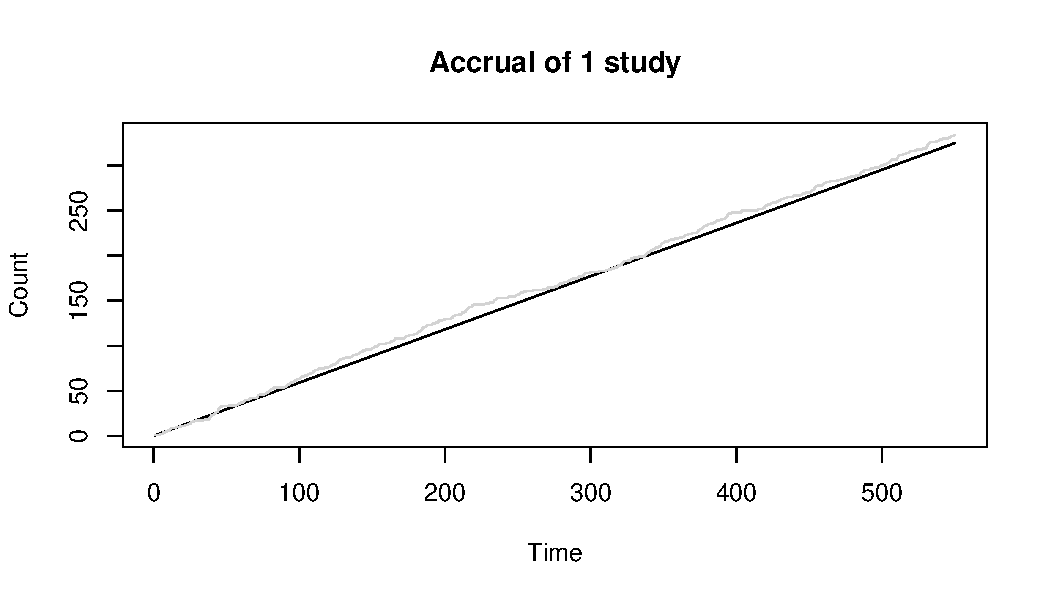
\includegraphics[width=\maxwidth]{figures/figunnamed-chunk-2-1} 
\end{knitrout}
 
\end{figure}


\end{frame}

\begin{frame}{Accrual of 2 studies}

\begin{figure}

\begin{knitrout}
\definecolor{shadecolor}{rgb}{0.969, 0.969, 0.969}\color{fgcolor}
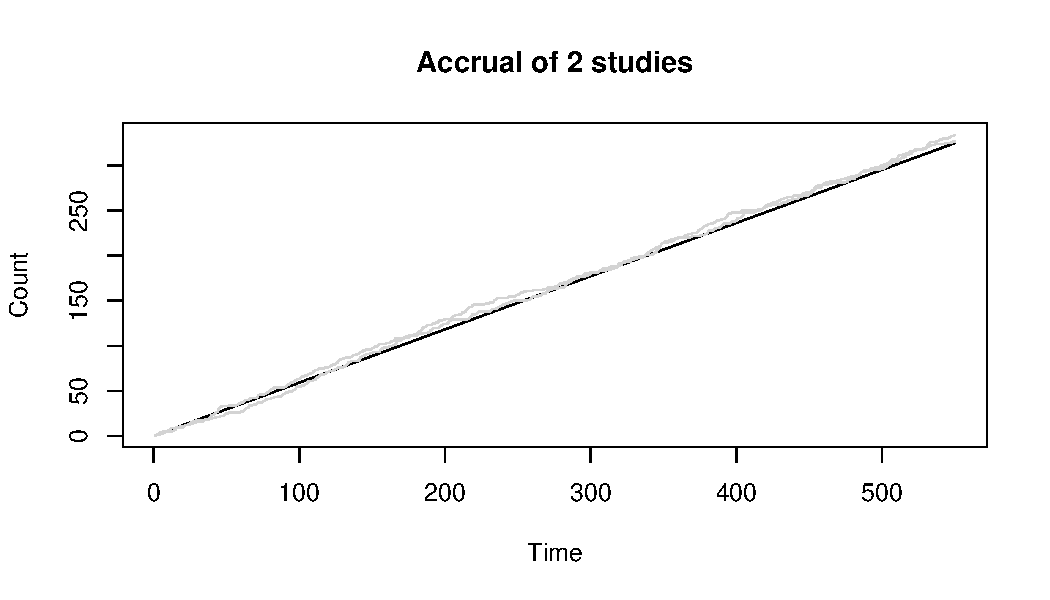
\includegraphics[width=\maxwidth]{figures/figunnamed-chunk-3-1} 
\end{knitrout}
  
\end{figure}


\end{frame}

\begin{frame}{Accrual of 100 studies}

\begin{figure}
\begin{knitrout}
\definecolor{shadecolor}{rgb}{0.969, 0.969, 0.969}\color{fgcolor}
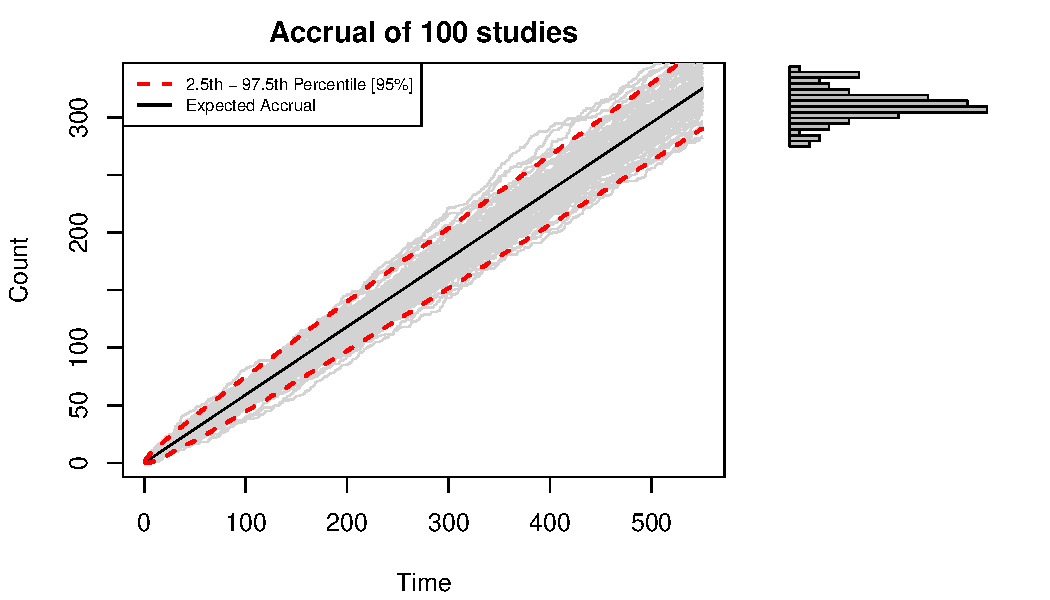
\includegraphics[width=\maxwidth]{figures/figunnamed-chunk-4-1} 
\end{knitrout}

\end{figure}

\end{frame}


\begin{frame}{Poisson's theoretical PMF}
\begin{figure}
\begin{knitrout}
\definecolor{shadecolor}{rgb}{0.969, 0.969, 0.969}\color{fgcolor}
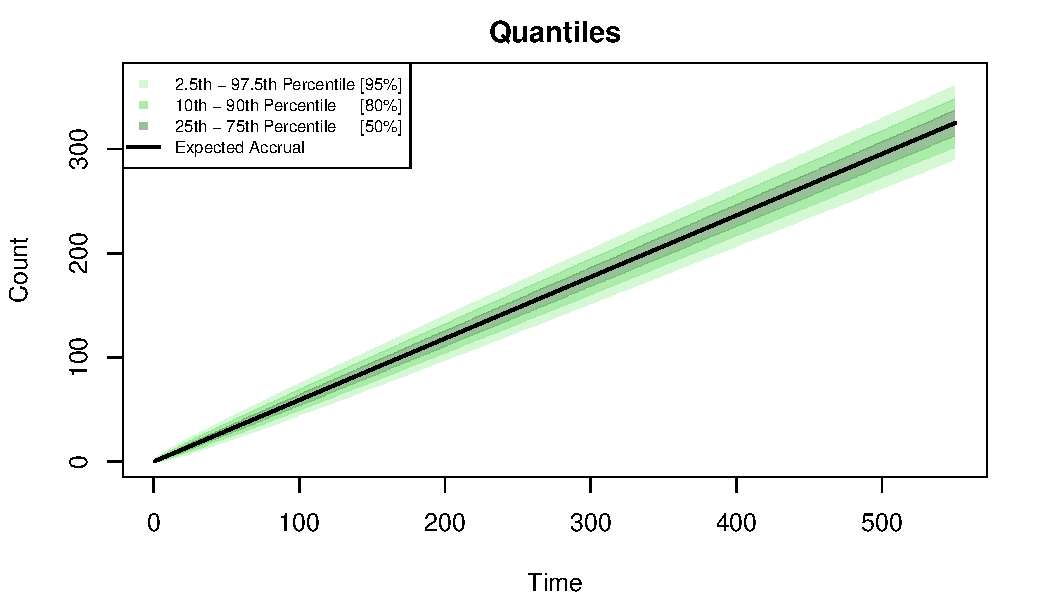
\includegraphics[width=\maxwidth]{figures/figunnamed-chunk-5-1} 
\end{knitrout}
  \caption{Poisson Distribution of Counts: This bar plot represents the probability mass function (PMF) of counts ranging from 200 to 500, using a Poisson distribution with a rate parameter $\lambda = 0.591$ based on 550 time periods.}
  \label{fig:2_3}
\end{figure}
\end{frame}

\begin{frame}{Poisson's theoretical CDF}

\begin{figure}
\begin{knitrout}
\definecolor{shadecolor}{rgb}{0.969, 0.969, 0.969}\color{fgcolor}
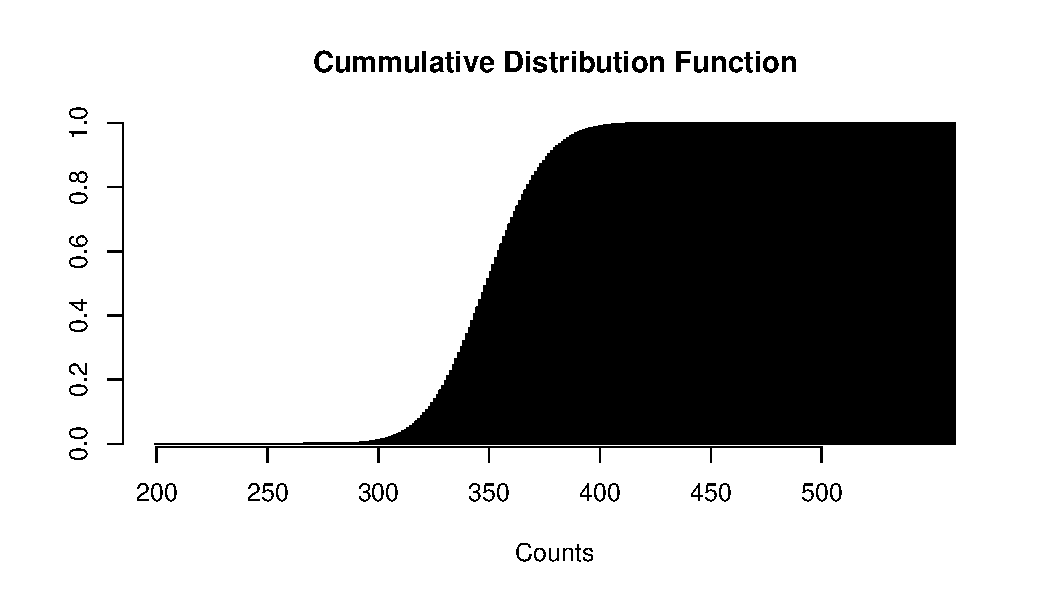
\includegraphics[width=\maxwidth]{figures/figunnamed-chunk-6-1} 
\end{knitrout}
  \caption{Cumulative Distribution of Poisson-Distributed Counts: The plot illustrates the cumulative probability distribution for counts within the range of 200 to 500, using a Poisson distribution with a rate parameter $\lambda = 0.591$ adjusted for 550 time periods.}
  \label{fig:2_4}
\end{figure}
\end{frame}

\begin{frame}{Poisson's uncertainty bands}


\begin{figure}
\begin{knitrout}
\definecolor{shadecolor}{rgb}{0.969, 0.969, 0.969}\color{fgcolor}
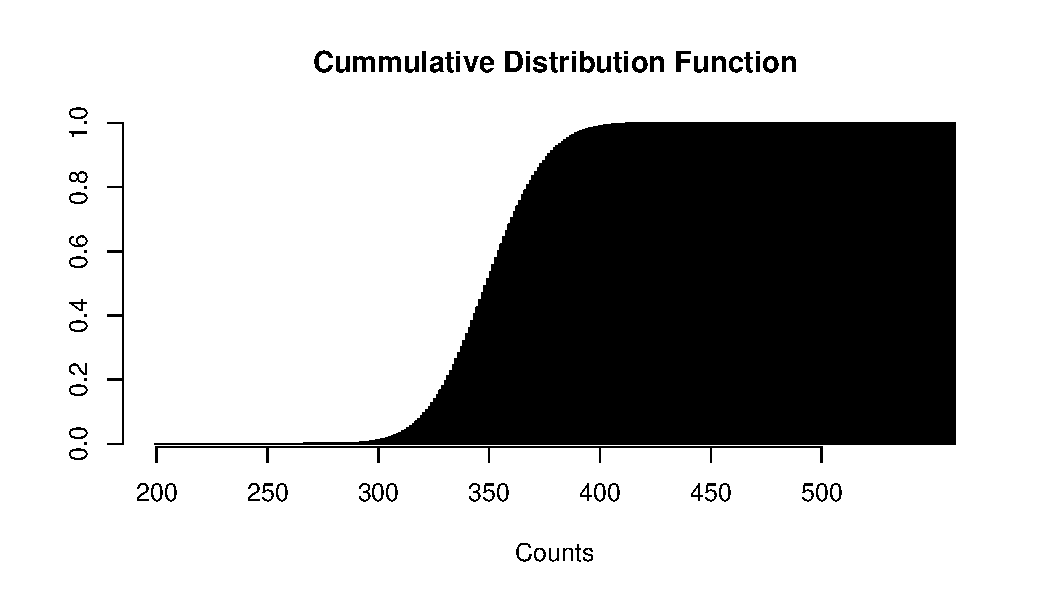
\includegraphics[width=\maxwidth]{figures/figunnamed-chunk-7-1} 
\end{knitrout}
\end{figure}

\end{frame}




\begin{frame}{A multicenter clinical trial evaluating the palliation benefits of radiation therapy and esophageal stents in subjects with terminal esophageal cancer}
\begin{itemize}
\item Time $t = 550$ days
\item Recruitment Rate $\lambda = \frac{Counts}{Time} = 0.591$
\item Models for Counts:
	\begin{itemize}
	\item Expectation: $\textrm{E}C(t) = \lambda t = 0.591 \cdot 550 = 325$
	\item \textbf{Poisson}: $C(t) \sim \textrm{Po}(\lambda t)$
	\item \textbf{Negative Binomial}: $C(t) \sim \textrm{Po} (\Lambda t)$; $\Lambda \sim \textrm{G}(\alpha,\beta)$
		\begin{itemize}
		\item $\alpha = 325$
		\item $\beta = 1.5\cdot 365$
		\item $\textrm{E} \Lambda = \frac{\alpha}{\beta} = 0.591 = \lambda$
		\end{itemize}
	\end{itemize}
\end{itemize}
\end{frame}

\begin{frame}[shrink = 5]{Negative binomial derived from Poisson-Gamma model (t=1)}

Let $C|\Lambda \sim \textrm{Po}(\Lambda)$ and $\Lambda \sim \textrm{G}(\alpha,\beta)$
\begin{align*}
p(c)&=\int^\infty_0 p(c|\lambda) p(\lambda) d\lambda\\
&=\int^\infty_0 \frac{\lambda^c\exp(-\lambda)}{c!}\Bigg[\lambda^{\alpha-1}\exp(-\beta\lambda)\frac{\beta^\alpha}{\Gamma(\alpha)}\Bigg]d\lambda\\
&=\frac{\beta^\alpha}{c!\Gamma(\alpha)}\int^\infty_0 \lambda^{\alpha+c-1}\exp(-\lambda)\exp(-\lambda\beta)d\lambda\\
&=\frac{\beta^\alpha\Gamma(\alpha+c)}{c!\Gamma(\alpha) (\beta+1)^{\alpha+c}}\underbrace{\int^\infty_0 \frac{(\beta+1)^{\alpha+c}}{\Gamma(\alpha+c)} \lambda^{\alpha+c-1}\exp(-(\beta+1)\lambda)d\lambda}_{=1}\\
&=\beta^\alpha\binom{\alpha+c-1}{\alpha-1}\Bigg (\frac{1}{\beta+1}\Bigg)^{\alpha+c}\\
&=\binom{\alpha+c-1}{\alpha-1}\Bigg (\frac{1}{\beta+1}\Bigg)^{c} \Bigg(\frac{\beta}{\beta+1}\Bigg)^{\alpha}, \ C|\Lambda\sim \textrm{NBin} \Bigg(\alpha, \frac{\beta}{\beta+1}\Bigg)
\end{align*}
\end{frame}


\begin{frame}{Expectation and Variance}
Using the expressions of iterated expectation and variance \citep{held2014applied}

\begin{align*}
\textrm{E}C &= \textrm{E}_{\Lambda}[\textrm{E}_{C} (C|\Lambda)] = \textrm{E}_{\Lambda}[\Lambda] = \alpha/\beta
\end{align*}

\begin{align*}
\textrm{Var}(C) &= \textrm{Var}_{\Lambda}[\textrm{E}_{C} (C|\Lambda)] + \textrm{E}_{\Lambda}[\textrm{Var}_C(C|\Lambda)]\\
&=\textrm{Var}_{\Lambda}[\Lambda] + \textrm{E}_{\Lambda}[\Lambda] \\
&=\alpha/\beta^2 + \alpha/\beta = \frac{\alpha(\beta+1)}{\beta^2}
\end{align*}
\end{frame}

\begin{frame}{Gamma Prior}
$\Lambda \sim \textrm{G}(\alpha,\beta)$
\begin{knitrout}
\definecolor{shadecolor}{rgb}{0.969, 0.969, 0.969}\color{fgcolor}
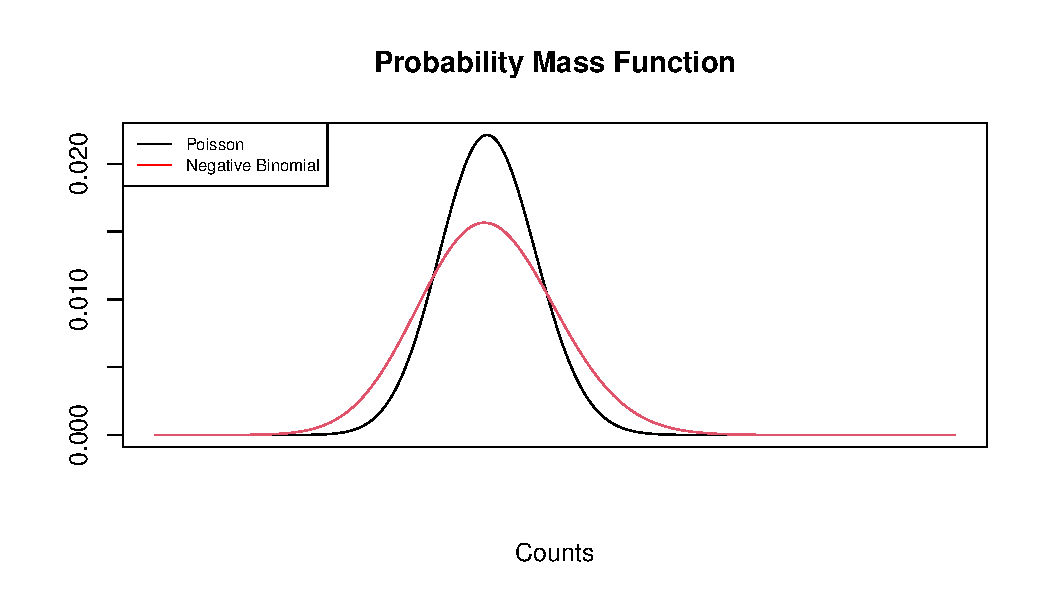
\includegraphics[width=\maxwidth]{figures/figunnamed-chunk-8-1} 
\end{knitrout}

\end{frame}


\begin{frame}{Comparison between Poisson and Negative Binomial}
\begin{figure}
\begin{knitrout}
\definecolor{shadecolor}{rgb}{0.969, 0.969, 0.969}\color{fgcolor}
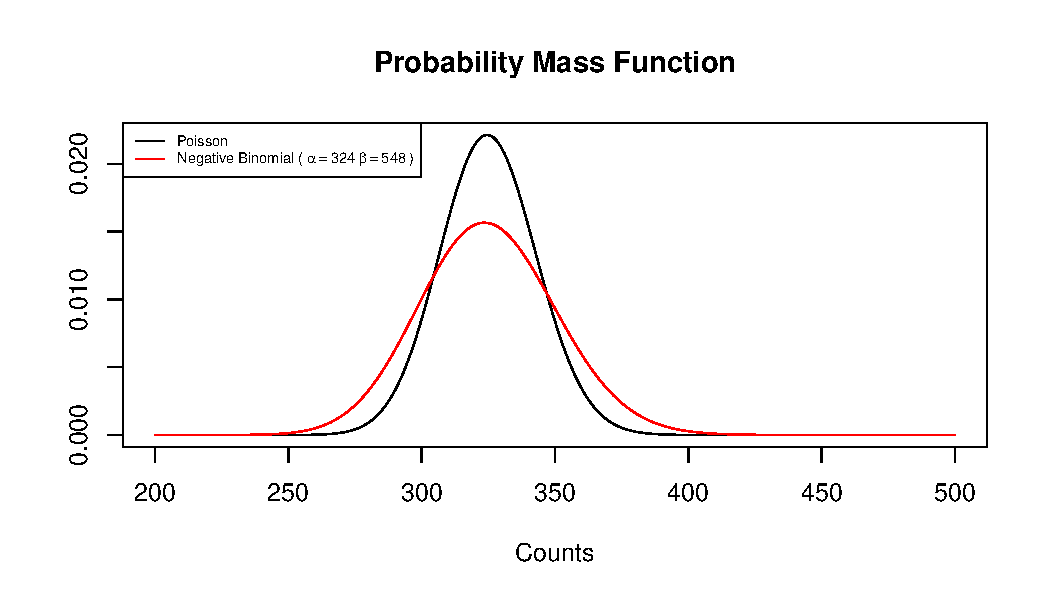
\includegraphics[width=\maxwidth]{figures/figunnamed-chunk-9-1} 
\end{knitrout}
  \caption{Comparison of Probability Mass Function (PMF) between Poisson distribution with $\lambda = 0.591$ and Negative Binomial with $\alpha = 324$ and $\mu = 0.591$.}
  \label{fig:2_6}
\end{figure}
\end{frame}


\begin{frame}{Comparison between Poisson and Negative Binomial}

\begin{figure}
\begin{knitrout}
\definecolor{shadecolor}{rgb}{0.969, 0.969, 0.969}\color{fgcolor}
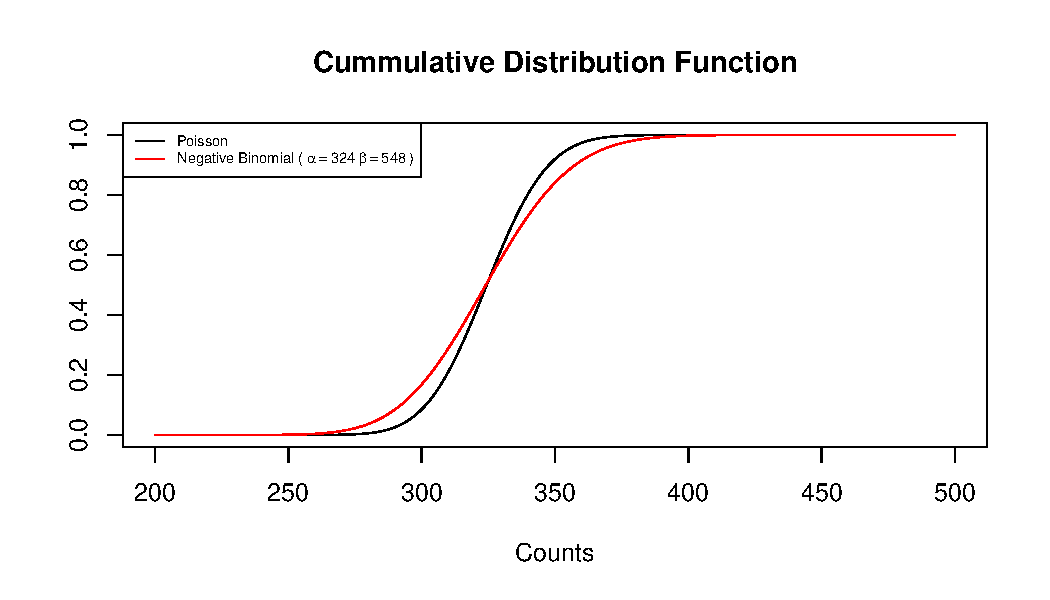
\includegraphics[width=\maxwidth]{figures/figunnamed-chunk-10-1} 
\end{knitrout}
  \caption{Comparison of Cummulative Distribution Function (CDF) between Poisson distribution with $\lambda = 0.591$ and Negative Binomial with $\alpha = 324$ and $\mu = 0.591$.}
  \label{fig:2_7}
\end{figure}

\end{frame}

\begin{frame}{Sensitivity Analysis}


\end{frame}


\begin{frame}{Sensitivity Analysis}
\begin{knitrout}
\definecolor{shadecolor}{rgb}{0.969, 0.969, 0.969}\color{fgcolor}
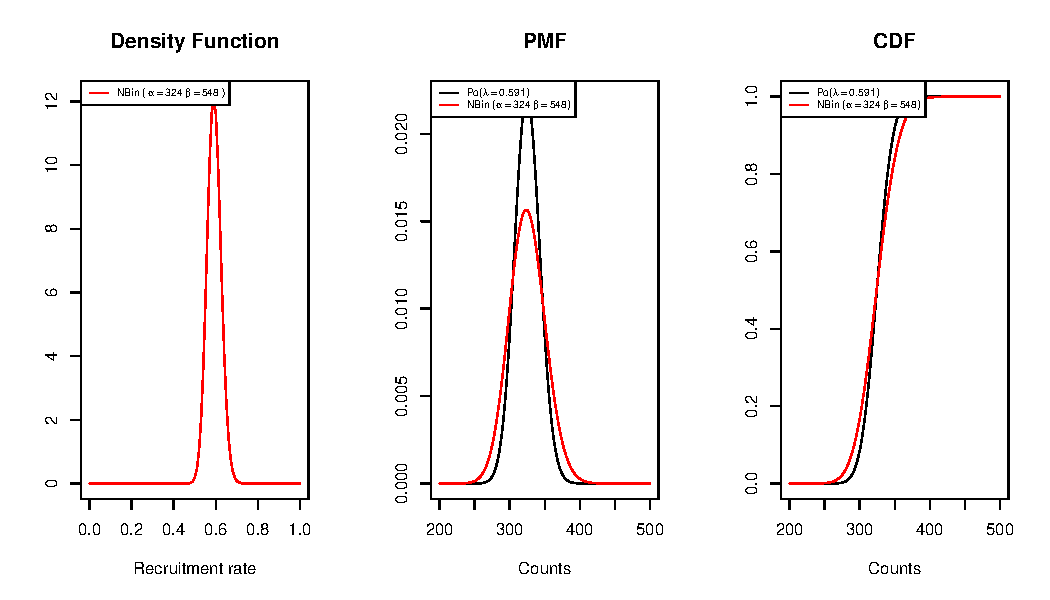
\includegraphics[width=\maxwidth]{figures/figunnamed-chunk-11-1} 
\end{knitrout}

\end{frame}


\begin{frame}{Sensitivity Analysis}
\begin{knitrout}
\definecolor{shadecolor}{rgb}{0.969, 0.969, 0.969}\color{fgcolor}
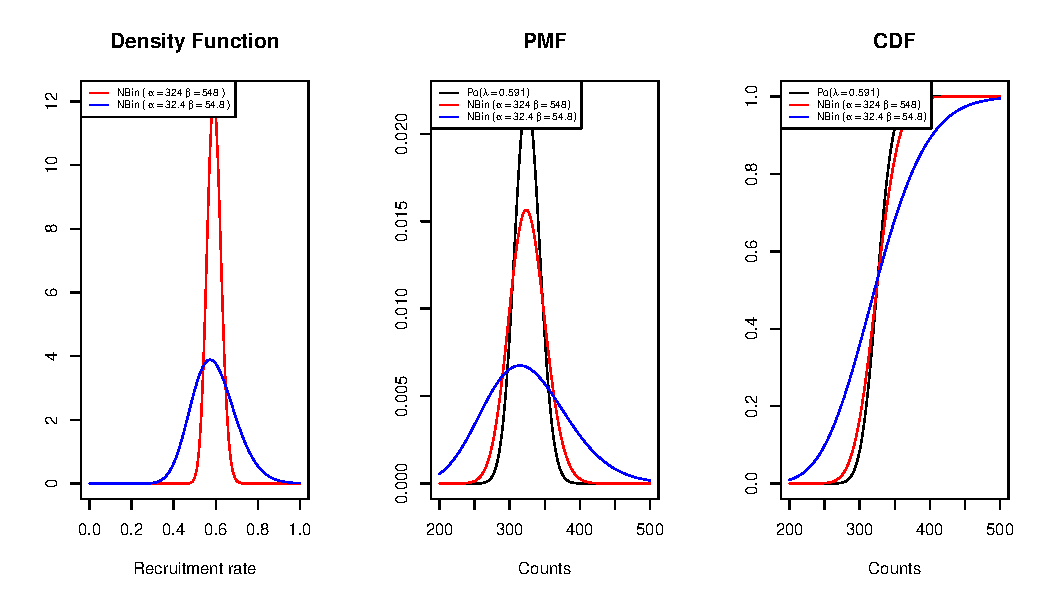
\includegraphics[width=\maxwidth]{figures/figunnamed-chunk-12-1} 
\end{knitrout}

\end{frame}



\begin{frame}{Sensitivity Analysis}
\begin{knitrout}
\definecolor{shadecolor}{rgb}{0.969, 0.969, 0.969}\color{fgcolor}
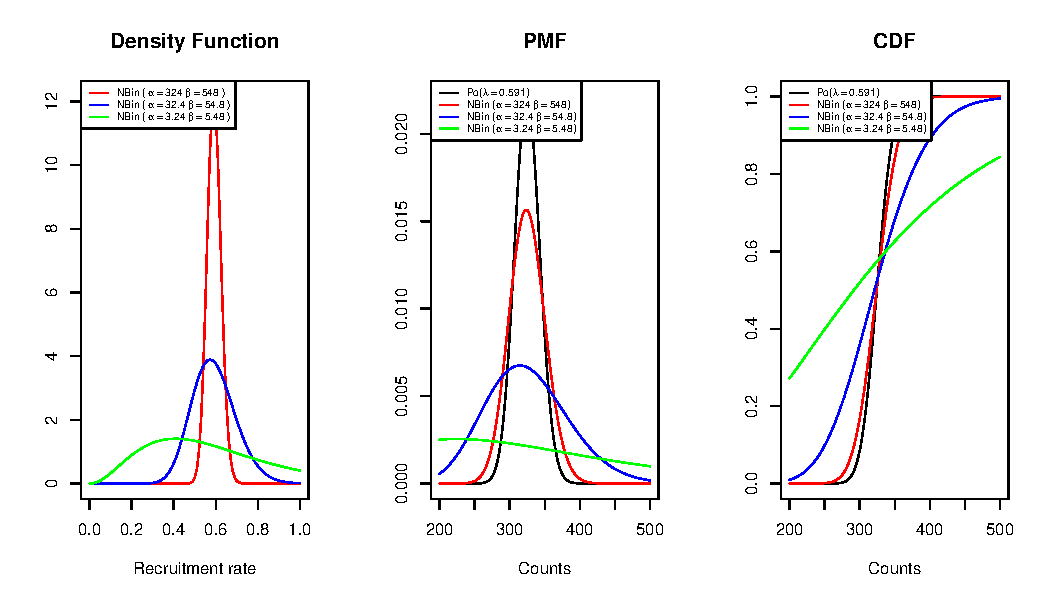
\includegraphics[width=\maxwidth]{figures/figunnamed-chunk-13-1} 
\end{knitrout}

\end{frame}




\begin{frame}{Summary}
\begin{itemize}
\item Theoretical models for \textbf{counts}
\item Extended Carter's simulation to exact distributions
\item Unified notation
\item Visualization of study accrual and uncertainty bands 
\end{itemize}

\end{frame}


\begin{frame}{Next steps}
\begin{itemize}
\item Application to simulation on \cite{carter2004application}
\item Models for \textbf{time} 
	\begin{itemize}
	\item Theoretical
	\item Application on \cite{carter2004application}
	\end{itemize}
\item Shiny App
\item Predictions using theoretical models developed on Daniore Nittas dataset of rates (cite?)
\end{itemize}

\end{frame}

\begin{frame}{References}
  \small
  \bibliographystyle{apalike}
\bibliography{illustration}
\end{frame}



%\appendix
%% Possible backup slides...

%% chapter division is accomplished with:
%% \part{Appendix}

\end{document}
